% ============================================================
%  Chapitre 2 : Compréhension métier et spécification des besoins
% ============================================================

\chapter{Compréhension métier et spécification des besoins}
\label{chap:business_understanding}

\section*{Introduction}
\addcontentsline{toc}{section}{Introduction}

Ce chapitre présente le contexte métier et les objectifs du projet d'assistant
intelligent de surveillance SAP dans le cadre de la méthodologie CRISP-DM. Il met en
évidence l'importance d'aligner les efforts techniques sur les objectifs métier, afin
que la solution développée réponde aux défis réels auxquels sont confrontées les équipes SAP.

Avant de commencer la phase de réalisation, il est crucial de bien définir les contours du système à mettre en place. Ce chapitre jette les bases du projet en identifiant les attentes des utilisateurs, en précisant les fonctionnalités requises et en établissant les contraintes à respecter. La méthodologie CRISP-DM oriente cette démarche structurée, depuis la compréhension du domaine jusqu'à la conception d'une solution appropriée pour le contexte de surveillance SAP d'Avaxia Group.

% ============================================================
\section{Contexte métier SAP}
\label{sec:contexte_sap}

\subsection{Qu'est-ce qu'un ERP ?}

Un système ERP (\textit{Enterprise Resource Planning}) est un logiciel qui intègre et
gère les principaux processus métier d'une organisation : finances, ressources humaines,
fabrication, chaîne d'approvisionnement, ventes et achats. Il fournit une source unique
de vérité, élimine la duplication des données et améliore l'efficacité opérationnelle.
Les solutions ERP permettent aux entreprises d'obtenir une visibilité en temps réel sur
leurs opérations, d'automatiser les processus et de prendre des décisions basées sur
les données.

\textbf{SAP} (\textit{Systems, Applications and Products in Data Processing}) est l'un
des principaux fournisseurs de logiciels ERP. Sa suite logicielle couvre de nombreux
domaines fonctionnels. Parmi ses modules les plus utilisés :

\begin{itemize}[leftmargin=*, label=\textbullet]
  \item \textbf{SAP EWM (\textit{Extended Warehouse Management}) :} Module spécialisé
        dans l'optimisation des entrepôts et la gestion des stocks. Il aide les entreprises
        à gérer efficacement leurs opérations d'entreposage et à garantir la disponibilité
        des produits au bon moment.
  \item \textbf{SAP ECC (\textit{Enterprise Central Component}) :} Module central de
        l'ERP SAP. Il intègre les finances, les ventes, les achats, la fabrication et
        les ressources humaines au sein d'une plateforme unifiée.
  \item \textbf{SAP Solution Manager (SOLMAN) :} Outil central de gestion et de
        surveillance fourni par SAP. Il couvre la gestion du cycle de vie des applications,
        la gestion de projets, la gestion des services IT et le suivi des processus métier.
\end{itemize}

\begin{figure}[H]
  \centering
  
\includegraphics[width=0.15\textwidth]{images/SAP_2011_logo.svg}
  \caption{Logo SAP}
  \label{fig:sap_logo}
\end{figure}

% ============================================================
\subsection{Le consultant SAP BASIS}

Le consultant SAP BASIS est responsable de l'infrastructure technique de l'environnement SAP : installations, mises à jour et application des correctifs. Il assure la résolution des problèmes de connectivité, les ajustements de composants et l'assistance aux systèmes externes et aux bases de données.

Ses principales responsabilités englobent l'administration des systèmes, la surveillance des performances, la sécurité et la gestion des bases de données, ainsi que la résolution des incidents techniques.

Il prend également en charge la sauvegarde et la récupération des données, la gestion des intégrations et des interfaces, les mises à jour et migrations des systèmes, et veille à maintenir une documentation à jour tout en assurant la formation des équipes concernées.

Dans le cadre du suivi opérationnel, il surveille en continu les performances et le bon fonctionnement des systèmes SAP à l'aide des transactions \textit{(T-Codes)} dédiées, et applique les correctifs nécessaires via les \textit{SAP Notes} afin de garantir la stabilité et la fiabilité de l'environnement.

% ============================================================
\subsection{Les codes de transaction SAP (T-codes)}

Dans SAP, les codes de transaction (T-codes) sont des commandes alphanumériques courtes
permettant d'accéder rapidement à des fonctions spécifiques, des rapports ou des
diagnostics système. Ils servent de points d'entrée dans les modules fonctionnels de SAP,
permettant aux utilisateurs de contourner les menus profonds et d'exécuter directement
des tâches telles que la surveillance des jobs, la gestion des files d'attente ou
l'analyse des performances.

Chaque T-code correspond à une fonction ou un programme backend : généralement implémenté
en ABAP : qui effectue un ensemble défini d'opérations. Lors de l'exécution d'un T-code,
SAP vérifie les autorisations de l'utilisateur, exécute la logique associée et présente
une interface interactive.

Dans le cadre de ce projet, un ensemble de T-codes à haute criticité a été sélectionné
pour assurer une couverture complète du comportement des systèmes SAP :

\begin{itemize}[leftmargin=*, label=\textbullet]
  \item \texttt{ST22} – Analyse des erreurs d'exécution ABAP (\textit{short dumps}).
  \item \texttt{DB02} – Surveillance des statistiques de base de données (croissance,
        espace table, index manquants).
  \item \texttt{SM37} – Surveillance des jobs en arrière-plan.
  \item \texttt{SP01} – Vérification des requêtes d'impression et de leurs statuts.
  \item \texttt{SM66} – Vue globale des processus de travail actifs.
  \item \texttt{SM58} – Analyse des erreurs RFC transactionnelles (traitement asynchrone).
  \item \texttt{SMQ1}, \texttt{SMQ2} – Surveillance des files d'attente entrantes et
        sortantes (qRFC/tRFC).
  \item \texttt{SM12}, \texttt{SM13} – Révision des entrées verrouillées et des
        enregistrements de mise à jour.
  \item \texttt{ST03N} – Analyse des statistiques de charge de travail et de performance.
  \item \texttt{SOST} – Surveillance des messages SAPconnect (e-mails, fax, etc.).
  \item \texttt{ST13} – Outils BASIS pour les diagnostics approfondis et les journaux.
\end{itemize}

Ces T-codes ont été sélectionnés en raison de leur criticité pour les opérations en temps
réel, de leur pertinence pour les équipes BASIS et de leur fréquence d'utilisation lors
de la résolution des incidents. En s'appuyant sur la documentation officielle de ces
transactions et sur les SAP Notes associées, le système permet aux consultants BASIS de
retrouver rapidement les procédures d'analyse et de résolution applicables à chaque
erreur observée.

\subsubsection*{SM37 : Job Overview}

SM37 surveille les \textit{jobs batch} — ce sont des tâches automatiques qui
tournent en arrière-plan (traitements de données, interfaces, rapports).
L'administrateur vérifie qu'aucun job n'est en erreur ou bloqué.

\begin{figure}[H]
  \centering
  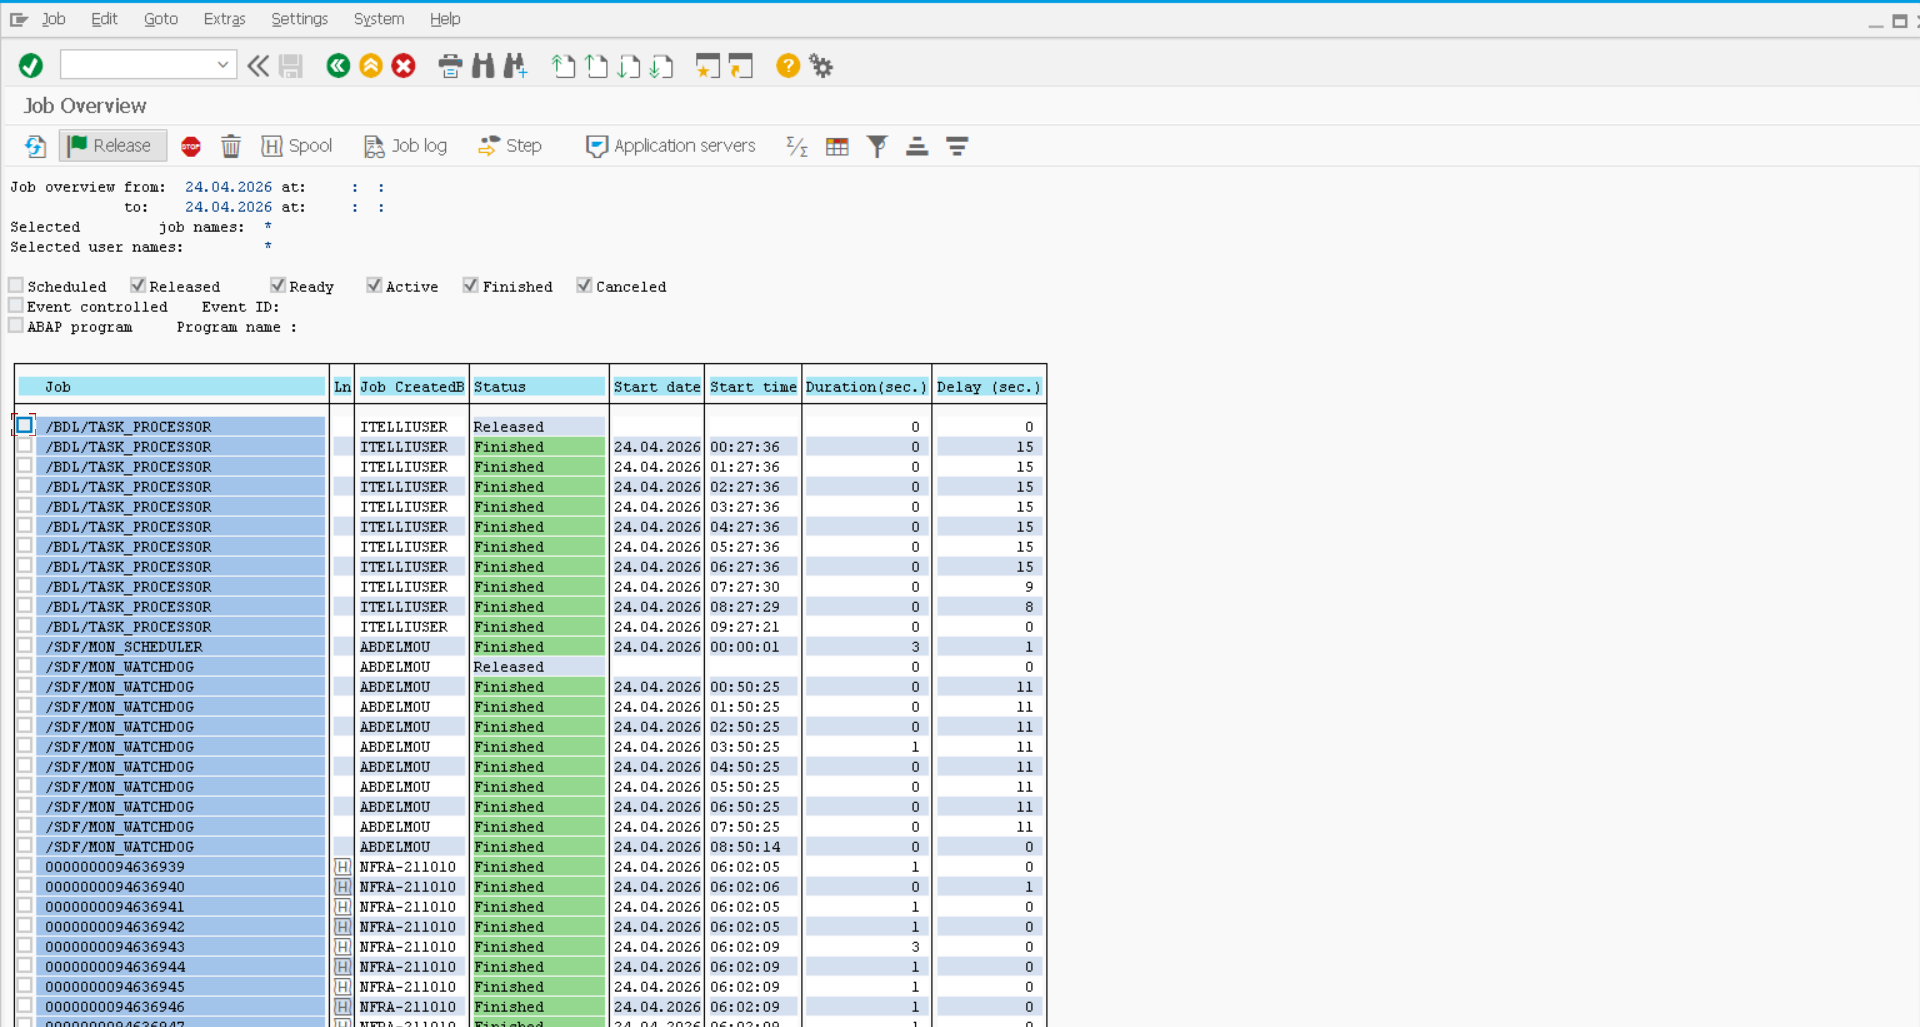
\includegraphics[width=\textwidth]{images/sm37.png}
  \caption{SM37 : Vue d'ensemble des jobs batch}
  \label{fig:sm37}
\end{figure}

La figure~\ref{fig:sm37} présente l'interface du T-code \texttt{SM37}, qui affiche
la liste des jobs planifiés avec leur statut (\textit{Finished}, \textit{Released},
\textit{Active}), leur date et heure de démarrage, leur durée d'exécution ainsi que
le délai éventuel. Cette vue permet à l'administrateur BASIS d'identifier en un coup
d'œil tout job bloqué, annulé ou présentant un délai anormal, et d'intervenir
rapidement avant que cela n'impacte les processus métier.

\subsubsection*{DB02 : Space Overview}

DB02 surveille la base de données ; l'administrateur contrôle l'espace disque
disponible pour éviter que la base de données sature, ce qui provoquerait un
arrêt complet du système.

\begin{figure}[H]
  \centering
  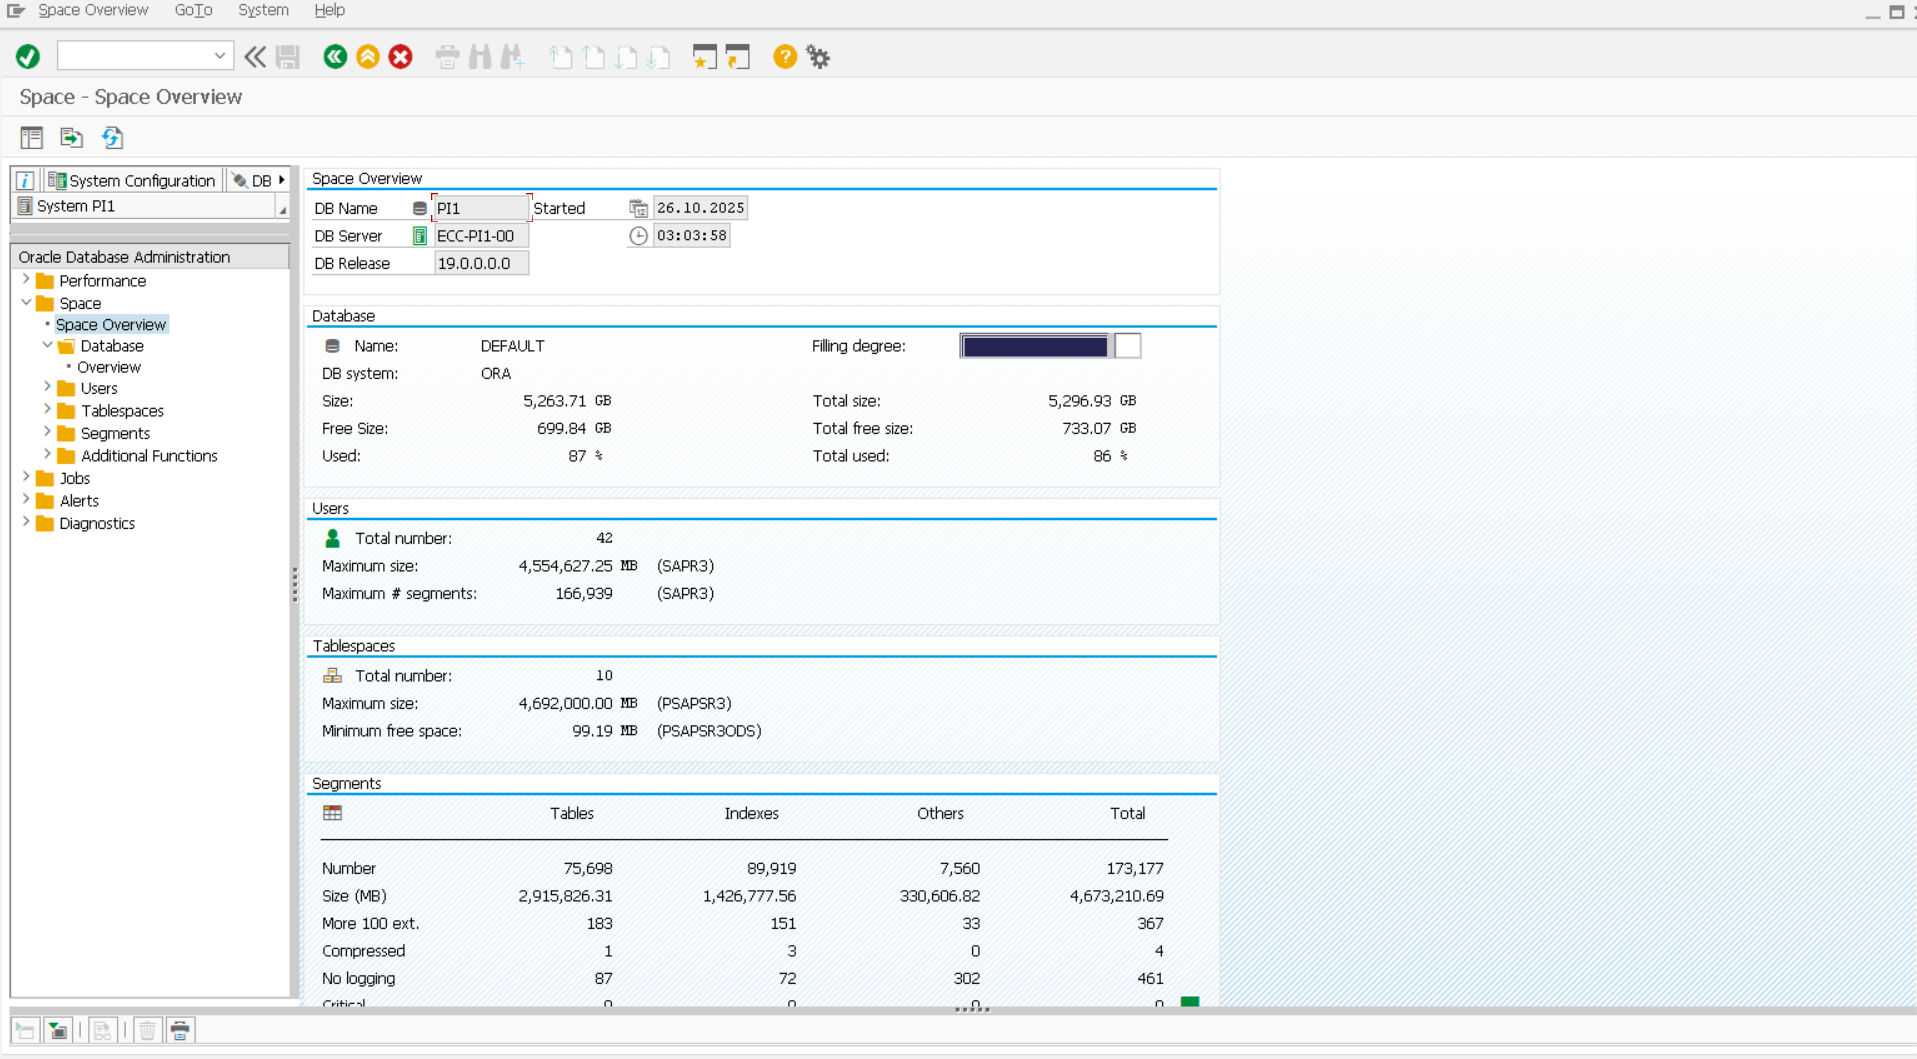
\includegraphics[width=\textwidth]{images/db02.png}
  \caption{DB02 : Vue d'ensemble de l'espace base de données}
  \label{fig:db02}
\end{figure}

La figure~\ref{fig:db02} illustre le T-code \texttt{DB02}, qui fournit une vue
synthétique de l'état de la base de données Oracle. On y retrouve le taux de
remplissage global, la taille totale et l'espace libre, ainsi que le détail par
tablespace et par segment (tables, index, autres). Un taux d'utilisation élevé
comme les 87\% visibles ici : constitue un signal d'alerte critique nécessitant
une action immédiate d'extension ou de purge pour prévenir toute saturation du système.

\subsubsection*{ST22 : Runtime Errors}

ST22 liste les erreurs critiques ABAP : l'administrateur analyse les
\textit{dumps} pour identifier les programmes qui plantent et corriger
les problèmes avant qu'ils n'impactent les utilisateurs.

\begin{figure}[H]
  \centering
  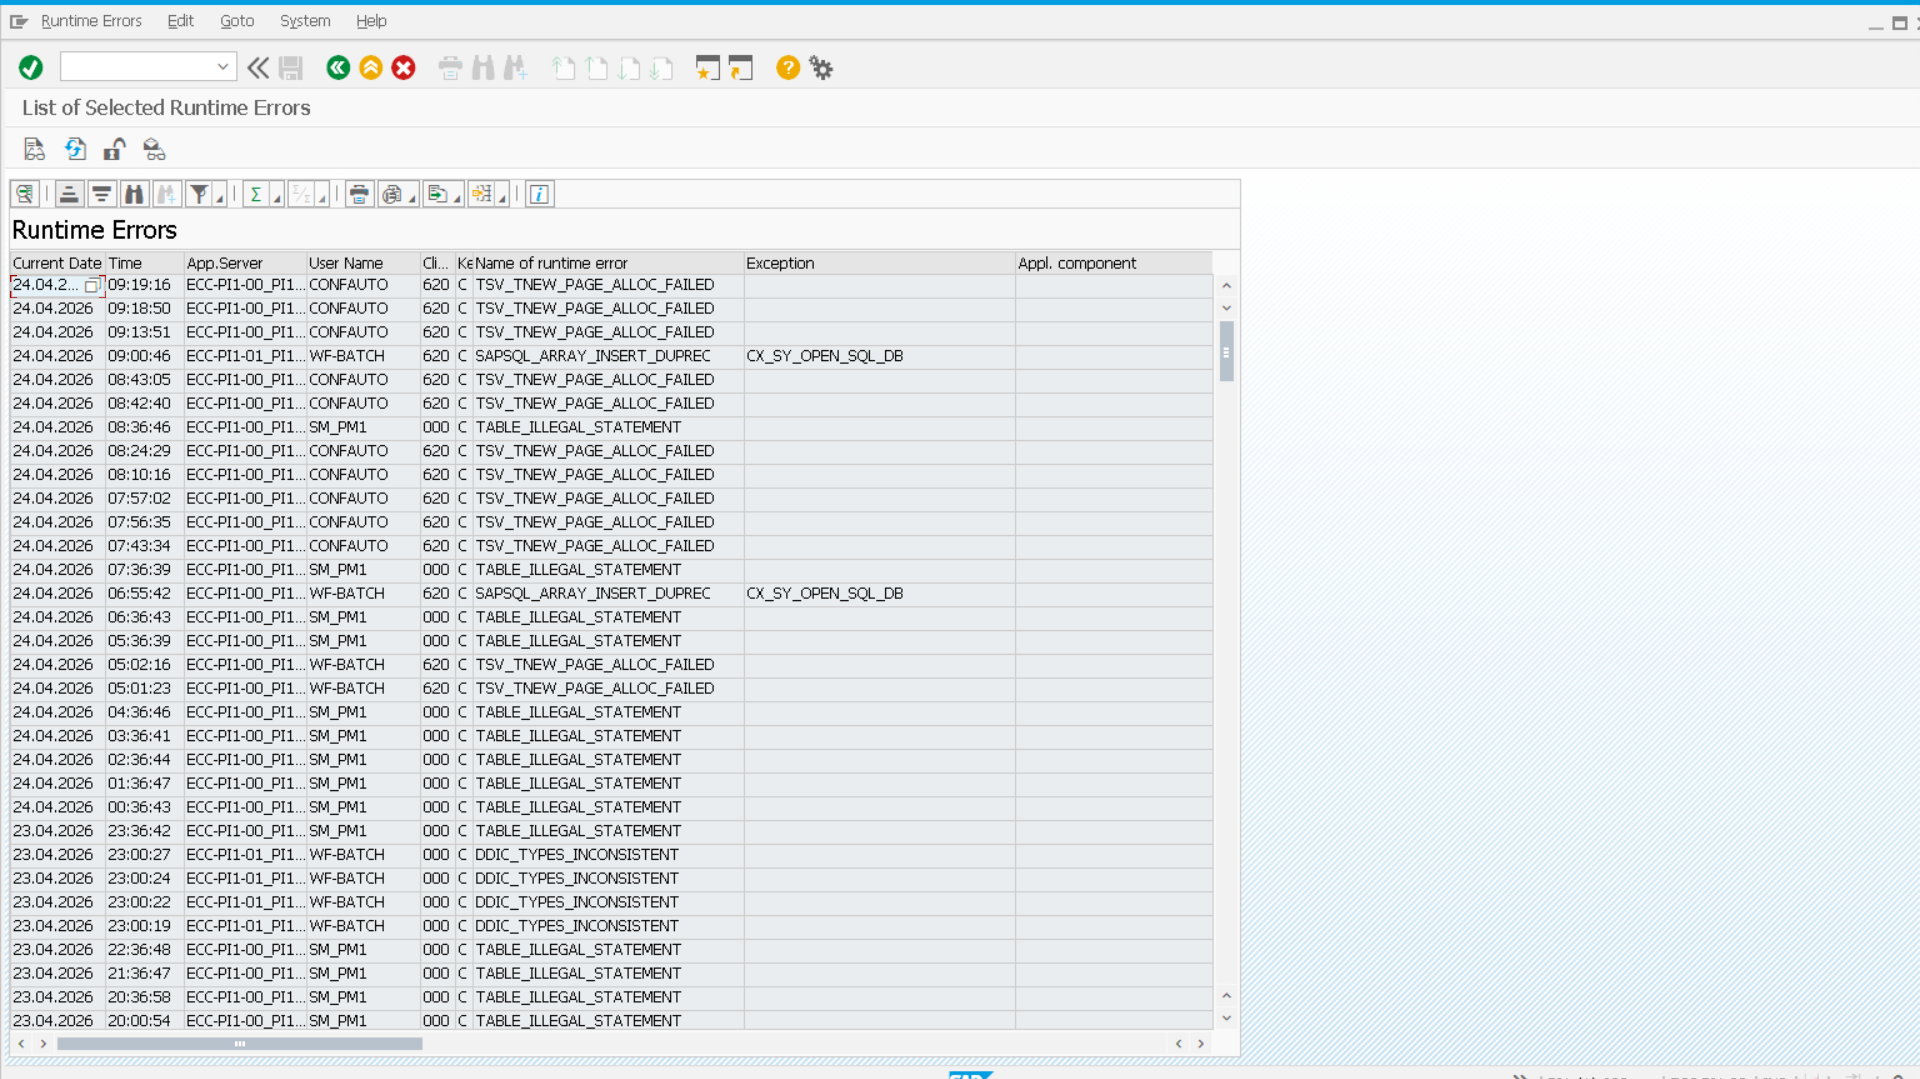
\includegraphics[width=\textwidth]{images/st22.png}
  \caption{ST22 : Liste des erreurs d'exécution ABAP}
  \label{fig:st22}
\end{figure}

La figure~\ref{fig:st22} présente l'interface du T-code \texttt{ST22}, qui recense
l'ensemble des \textit{short dumps} ABAP survenus sur le système. Chaque entrée
indique la date, l'heure, le serveur applicatif, l'utilisateur concerné et le nom
de l'erreur. Les erreurs récurrentes telles que \texttt{TSV\_TNEW\_PAGE\_ALLOC\_FAILED}
(manque de mémoire) ou \texttt{TABLE\_ILLEGAL\_STATEMENT} (instruction SQL non autorisée)
sont des indicateurs d'anomalies systémiques qui doivent être analysées et résolues
en priorité par l'équipe BASIS.

% ─────────────────────────────────────────────────────────────
\section{Vision et objectifs du système futur}
% ─────────────────────────────────────────────────────────────

Dans le cadre de l'optimisation et de la modernisation de l'exploitation des systèmes SAP, le projet vise à développer un assistant intelligent capable d'analyser et d'exploiter de manière efficace les données issues des différentes transactions et opérations. Les principaux objectifs du système futur sont les suivants :

\begin{itemize}
    \item \textbf{Centraliser et organiser les données SAP} provenant des différents modules, afin de disposer d'une source unique et fiable d'informations.
    \item \textbf{Analyser et interpréter les incidents} grâce à un assistant intelligent qui retrouve et présente les procédures de diagnostic et de résolution adaptées au contexte SAP de l'utilisateur.
    \item \textbf{Faciliter l'analyse des incidents} en fournissant rapidement, à partir d'un T-code ou d'un message d'erreur, les sections de documentation et les SAP Notes pertinentes pour leur résolution.
    \item \textbf{Exploiter le corpus documentaire SAP} grâce à un pipeline de recherche sémantique et lexicale (RAG hybride), produisant des réponses sourcées et vérifiables en langage naturel.
    \item \textbf{Offrir une interface interactive} sous forme d'assistant conversationnel permettant aux utilisateurs de poser des questions, d'obtenir des analyses et de recevoir des conseils personnalisés.
    \item \textbf{Assurer une accessibilité via une application web} intuitive, permettant de visualiser les analyses, exploiter les données collectées et interagir avec l'assistant de manière ergonomique.
\end{itemize}

Ainsi, ce système contribuera à améliorer la compréhension et la gestion des données SAP, à faciliter l'analyse des anomalies, et à offrir un outil intelligent d'aide à la décision pour les utilisateurs.

% ─────────────────────────────────────────────────────────────
\section{Spécification des besoins}
\label{sec:specification_besoins}
% ─────────────────────────────────────────────────────────────

L'analyse des besoins a pour objectif de comprendre les attentes des utilisateurs et de définir le
contexte métier dans lequel s'inscrit le système à développer. Elle permet de décrire
les fonctionnalités que le système prendra en charge, ses interactions avec les différents
intervenants, ainsi que les règles qui encadrent ces interactions.

\subsection{Identification des acteurs}

Pour déterminer les besoins fonctionnels et non fonctionnels, nous débutons par
l'identification des acteurs impliqués dans le système, en précisant le rôle spécifique
de chacun. Ainsi, nous identifions trois rôles distincts qui interagissent avec le
système :

\begin{table}[H]
\centering
\renewcommand{\arraystretch}{1.45}
\caption{Acteurs du système AutoMoni et leurs responsabilités}
\label{tab:acteurs}
\begin{tabularx}{\textwidth}{|p{4.5cm}|p{3.5cm}|X|}
\hline
\textbf{Acteur} & \textbf{Type} & \textbf{Responsabilités principales} \\
\hline
Administrateur SAP (consultant BASIS)
  & Acteur principal
  & Surveille les environnements SAP à travers les données de monitoring collectées en temps réel. Interagit avec l'assistant intelligent pour poser des questions techniques en langage naturel, consulter les alertes T-code, accéder aux journaux de transactions et visualiser les graphiques d'analyse. Configure les paramètres de surveillance et de la plateforme AutoMoni. Soumet des feedbacks sur les réponses du chatbot afin d'améliorer la qualité du système RAG. Cumule l'ensemble des privilèges de l'Utilisateur SAP. \\
\hline
Utilisateur SAP
  & Acteur principal
  & Consulte les pages de monitoring SAP, interagit avec l'assistant intelligent via la page chatbot ou le panneau latéral, pose des questions en langage naturel, navigue vers les pages T-code depuis le chatbot et consulte l'historique de ses conversations. \\
\hline
Système SAP (source externe)
  & Acteur secondaire
  & Fournit les données de surveillance opérationnelle via les appels RFC (PyRFC). Ne déclenche pas d'interactions directes avec l'interface, mais alimente en continu la base de données de monitoring interrogée par les acteurs humains. \\
\hline
\end{tabularx}
\end{table}

\subsection{Besoins fonctionnels}

Les besoins fonctionnels définissent l'ensemble des fonctionnalités que le système doit
fournir afin de permettre aux utilisateurs d'exploiter et d'analyser les données issues
de l'environnement SAP à travers un assistant intelligent basé sur l'intelligence
artificielle et reposant sur une architecture de génération augmentée par récupération
\textit{(RAG -- Retrieval-Augmented Generation)}.

Le système repose sur deux types d'acteurs principaux : l'\textbf{Administrateur SAP}
et l'\textbf{Utilisateur SAP}. Il convient de préciser que l'administrateur SAP englobe
l'ensemble des privilèges de l'utilisateur SAP : en plus de ses responsabilités de
supervision et de configuration, il peut également interagir avec l'assistant intelligent
et exploiter pleinement les fonctionnalités offertes par le module RAG, au même titre
qu'un utilisateur standard.

\subsubsection*{Administrateur SAP}

L'administrateur occupe un rôle central de supervision et de gouvernance de la plateforme AutoMoni.
En tant qu'acteur disposant des droits les plus étendus, il cumule l'ensemble des fonctionnalités
de l'utilisateur SAP, auxquelles s'ajoutent ses responsabilités d'administration.
Ses responsabilités spécifiques sont les suivantes~:

\begin{itemize}
  \item Interagir avec l'assistant intelligent RAG via la page chatbot dédiée ou le tiroir
        latéral accessible depuis toutes les pages.
  \item Formuler des requêtes en langage naturel sur les données SAP et recevoir des réponses
        vérifiées accompagnées de leurs sources documentaires.
  \item Naviguer automatiquement vers une page de monitoring en mentionnant un T-code dans le chatbot.
  \item Soumettre un retour (\textit{feedback}) sur les réponses générées afin d'améliorer
        la qualité du pipeline RAG.
\end{itemize}

\subsubsection*{Utilisateur SAP}

L'utilisateur SAP constitue l'acteur principal de l'application AutoMoni.
Il peut exploiter les fonctionnalités suivantes~:

\begin{itemize}
  \item S'authentifier à l'application.
  \item Consulter les pages de monitoring SAP correspondant aux T-codes de surveillance.
  \item Interagir avec l'assistant intelligent via la page chatbot dédiée ou via le panneau
        latéral coulissant disponible sur toutes les pages.
  \item Poser des questions en langage naturel sur les données issues du système SAP.
  \item Naviguer vers une page de monitoring en mentionnant un T-code dans le chatbot.
  \item Consulter les sources documentaires et les avertissements associés à chaque réponse.
  \item Consulter l'historique de ses propres interactions avec le chatbot.
\end{itemize}

\subsection{Besoins non fonctionnels}

Les besoins non fonctionnels définissent les critères de qualité mesurables que le système doit respecter. Ils constituent les \textit{Business Success Criteria} de la phase Business Understanding de CRISP-DM et seront confrontés aux mesures du chapitre~6.

\subsubsection{Performance}

Le pipeline complet (retrieval + génération) doit retourner une réponse en moins de 5 secondes pour 95\,\% des requêtes (P95 $\leq$ 5\,s). Ce seuil justifie le choix de l'index HNSW (recherche en $O(\log n)$) et le déploiement local du LLM via Ollama.

\subsubsection{Fiabilité}

Le taux d'hallucination doit rester inférieur à 5\,\%, garanti par une validation déterministe par règles~: les T-codes SAP et numéros de SAP Notes mentionnés dans la réponse sont comparés par expressions régulières à ceux présents dans les chunks récupérés~; toute entité non ancrée est supprimée avant renvoi (cf.\ §\,5.9.5 et §\,6.7).

\subsubsection{Confidentialité}

L'intégralité du pipeline tourne en local — LLM via Ollama, base vectorielle via PostgreSQL/pgvector. Aucune donnée SAP n'est transmise à des APIs cloud externes.

\subsubsection{Scalabilité}

L'index HNSW supporte l'insertion incrémentale sans reconstruction, ce qui permet d'ajouter de nouvelles SAP Notes ou de nouveaux modules sans réindexer l'intégralité du corpus.

\begin{table}[H]
\centering
\renewcommand{\arraystretch}{1.3}
\caption{Synthèse des besoins non fonctionnels}
\label{tab:nfr_synthese}
\begin{tabularx}{\textwidth}{|p{3cm}|p{4cm}|X|}
\hline
\textbf{Catégorie} & \textbf{Seuil cible} & \textbf{Mécanisme de garantie} \\
\hline
Performance & P95 $\leq$ 5\,s & Index HNSW + LLM local Ollama \\
\hline
Fiabilité & Taux d'hallucination $<$ 5\,\% & Validation ensembliste des T-codes et SAP Notes (§\,5.9.5, §\,6.7) \\
\hline
Confidentialité & 0 donnée transmise à des APIs cloud & Pipeline 100\,\% local (Ollama + pgvector) \\
\hline
Scalabilité & Insertion sans réindexation & Index HNSW incrémental (PostgreSQL pgvector) \\
\hline
\end{tabularx}
\end{table}

\subsection{Diagramme de cas d'utilisation général}

La figure~\ref{fig:usecase_deploy} synthétise les interactions entre les acteurs identifiés et les fonctionnalités du système. L'Administrateur SAP cumule les privilèges de l'Utilisateur SAP et y ajoute la configuration de la plateforme. L'Utilisateur SAP peut consulter les pages de monitoring, interroger l'assistant et naviguer automatiquement vers les pages T-code mentionnées dans les réponses.

\begin{figure}[H]
    \centering
    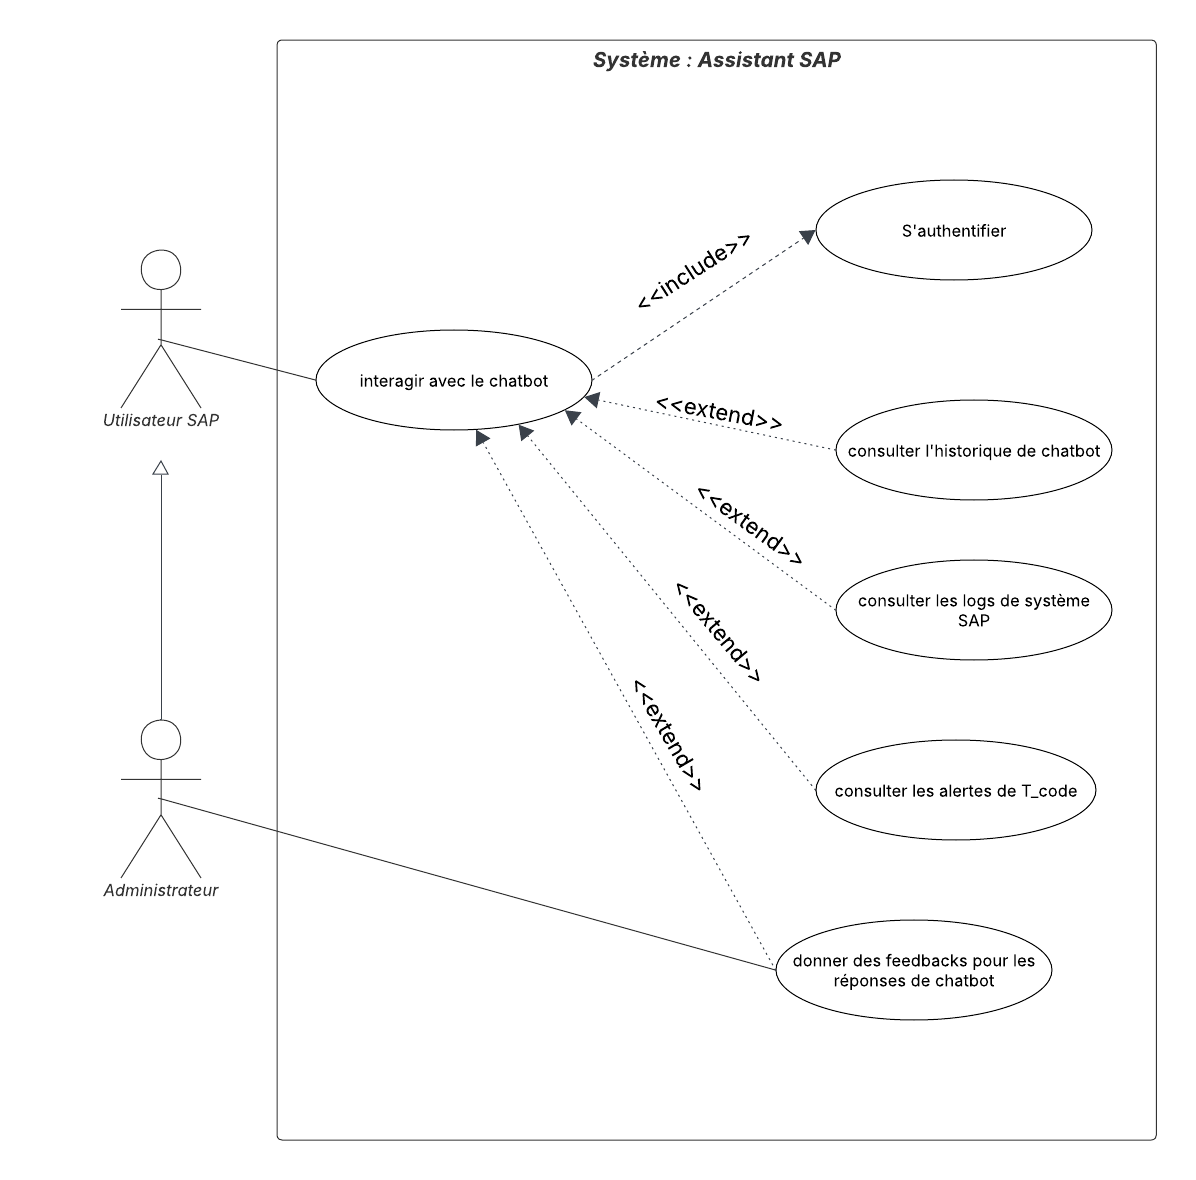
\includegraphics[width=0.9\textwidth]{images/casutilisation.png}
    \caption[Diagramme de cas d'utilisation]{Diagramme de cas d'utilisation général du système}
    \label{fig:usecase_deploy}
\end{figure}

% ============================================================
\section{État de l'art}
\label{sec:etat_art}

\subsection{Les Fondements Technologiques de l'IA Générative}

L'intelligence artificielle générative repose sur un ensemble de technologies complémentaires qui, combinées, permettent de concevoir des systèmes capables d'analyser, de raisonner et de produire du contenu à partir de données complexes. Cette section présente les principaux fondements technologiques qui soutiennent la compréhension et la génération du langage naturel.

Elle introduit tout d'abord les concepts essentiels de l'apprentissage automatique (\textit{Machine Learning}) et de l'intelligence artificielle, avant d'explorer l'apprentissage profond (\textit{Deep Learning}) ainsi que les modèles basés sur l'architecture \textit{Transformer}. Elle aborde ensuite le traitement automatique du langage naturel (\textit{NLP -- Natural Language Processing}) et met en lumière l'émergence des modèles de langage de grande taille (\textit{LLMs -- Large Language Models}), qui jouent un rôle central dans la génération de texte. Enfin, l'architecture \textit{RAG (Retrieval-Augmented Generation)} est présentée comme une approche permettant d'enrichir ces modèles en leur fournissant un accès à des connaissances actualisées et vérifiables. L'ensemble de ces technologies constitue le socle sur lequel repose la solution proposée dans ce projet.

\subsection{Machine Learning et Intelligence Artificielle}

Le \textit{Machine Learning}, ou apprentissage automatique, constitue l'un des piliers fondamentaux de l'intelligence artificielle. Il permet à un système d'apprendre à partir de données sans être explicitement programmé pour chaque tâche. En analysant des ensembles de données, le modèle identifie des régularités statistiques qu'il utilise pour effectuer des prédictions sur de nouvelles données. Cette capacité d'apprentissage automatique est à la base des avancées récentes en intelligence artificielle générative.

\subsection{Deep Learning}

L'apprentissage profond (\textit{Deep Learning}) est une sous-discipline du \textit{Machine Learning} qui repose sur des réseaux de neurones artificiels composés de plusieurs couches. Ces réseaux permettent d'extraire progressivement des représentations de plus en plus abstraites des données. Grâce à cette structure, ils sont particulièrement efficaces pour traiter des données non structurées telles que le texte, les images ou encore les signaux audio.

\subsection{Architecture Transformer}

Proposée en 2017 dans l'article \textit{« Attention is All You Need »} \cite{vaswani2017attention}, l'architecture \textit{Transformer} s'est imposée comme une référence dans le domaine du traitement du langage naturel. Elle repose sur le mécanisme d'\textbf{attention} (\textit{self-attention}), qui permet au modèle d'évaluer l'importance de chaque mot par rapport à tous les autres mots d'une séquence, indépendamment de leur position.

Contrairement aux architectures séquentielles traditionnelles telles que les réseaux récurrents (\textit{RNN, LSTM}), le Transformer traite les données en parallèle, ce qui améliore considérablement les performances et permet de capturer efficacement les dépendances à long terme dans le texte.

\subsection{Traitement Automatique du Langage Naturel (NLP)}

Le traitement automatique du langage naturel (\textit{NLP}) est un domaine de l'intelligence artificielle dédié à l'interaction entre les machines et le langage humain. Il regroupe un ensemble de techniques permettant de comprendre, analyser et générer du texte~\cite{jurafsky2024slp}.

Parmi les principales applications du NLP figurent la classification de textes, l'analyse de sentiments, la traduction automatique, la reconnaissance d'entités nommées ainsi que la génération automatique de contenu.

\subsection{Les Modèles de Langage de Grande Taille : Capacités et Limites}

Les modèles de langage de grande taille (\textit{LLMs}) sont des modèles avancés d'apprentissage profond entraînés sur des volumes massifs de données textuelles (livres, articles, sites web, code, etc.). Leur objectif est de comprendre et de générer un langage proche de celui des humains~\cite{brown2020gpt3}.

Comme illustré dans la figure~\ref{fig:llm_intersection}, ces modèles se situent à l'intersection du \textit{Deep Learning} et du \textit{NLP}, combinant ainsi la puissance des réseaux de neurones profonds avec les techniques d'analyse linguistique.

En pratique, un LLM prédit le mot (ou jeton) le plus probable à la suite d'une séquence donnée. En répétant ce processus, il est capable de produire des textes cohérents, de répondre à des questions, de résumer des documents ou encore de traduire des contenus. Plus le modèle contient de paramètres, plus il est capable de capturer les nuances complexes du langage.

\begin{figure}[H]
  \centering
  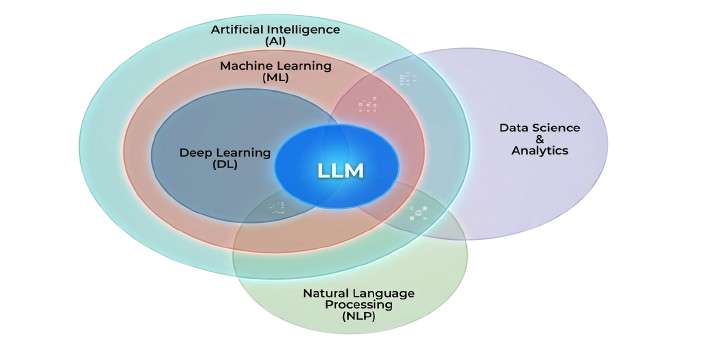
\includegraphics[width=0.6\textwidth]{images/llmv1.png}
  \caption{Les LLMs à l'intersection du \textit{Deep Learning} et du \textit{NLP}}
  \label{fig:llm_intersection}
\end{figure}

Malgré leurs performances impressionnantes, les LLMs présentent certaines limites. Leur connaissance est limitée aux données utilisées lors de leur entraînement, ce qui les empêche de traiter des informations récentes. De plus, ils peuvent générer des \textbf{hallucinations}, c'est-à-dire produire des réponses plausibles mais incorrectes. Enfin, ils n'ont pas accès aux données internes ou confidentielles d'une organisation.

Parmi les modèles les plus connus figurent \textit{GPT-4}, \textit{Claude} et \textit{Gemini}.

\subsection{Architecture de RAG (Retrieval-Augmented Generation)}

Bien que les LLMs possèdent une connaissance générale acquise lors de leur entraînement, ils ne disposent pas d'un accès direct aux données spécifiques d'une organisation ni aux informations les plus récentes. L'architecture \textit{RAG (Retrieval-Augmented Generation)}~\cite{lewis2020rag} a été conçue pour répondre à cette limitation.

Son fonctionnement repose sur plusieurs étapes. Tout d'abord, les documents sont découpés en fragments appelés \textit{chunks}. Chaque fragment est ensuite transformé en un vecteur numérique (\textit{embedding}) représentant son contenu sémantique~\cite{reimers2019sbert}. Ces vecteurs sont stockés dans une base de données vectorielle.

Lorsqu'une requête utilisateur est soumise, le système identifie les fragments les plus pertinents à l'aide d'une mesure de similarité (généralement la similarité cosinus). Ces informations sont ensuite injectées dans le contexte du modèle, qui génère une réponse basée sur des données réelles et vérifiables.

Ainsi, le RAG peut être comparé à un assistant intelligent capable de consulter une base documentaire avant de formuler une réponse, garantissant ainsi une meilleure fiabilité.
\begin{figure}[H]
\centering
\resizebox{\textwidth}{!}{
\begin{tikzpicture}[
    node distance=2.2cm and 1.6cm,
    every node/.style={font=\footnotesize},
    box/.style={
        draw,
        rounded corners=8pt,
        minimum width=2.6cm,
        minimum height=0.9cm,
        align=center,
        line width=0.8pt,
        drop shadow={opacity=0.15}
    },
    arrow/.style={->, line width=0.9pt}
]

% ---- NODES ----
\node[box, fill=SAPLightOrange, draw=SAPOrange] (docs) {Documents};

\node[box, fill=SAPLightBlue, draw=SAPBlue, right=of docs] (chunk) {Chunking};

\node[box, fill=gray!10, draw=black!50, right=of chunk] (query) {User Query};

\node[box, fill=SAPLightGreen, draw=SAPGreen, right=of query] (vectordb) {Vector DB};

\node[box, fill=SAPLightOrange, draw=SAPRed, below=1.8cm of vectordb] (retrieval) {Top-K\\Retrieval};

\node[box, fill=SAPLightOrange, draw=SAPOrange, left=of retrieval] (llm) {LLM};

\node[box, fill=SAPLightBlue, draw=SAPBlue, left=of llm] (response) {Response};

% ---- FLUX ----
\draw[arrow] (docs) -- node[above]{découpage} (chunk);

\draw[arrow] (chunk) -- node[above]{vectorisation} (query);

\draw[arrow, dashed, color=SAPGreen]
(query) -- node[above]{stockage} (vectordb);

\draw[arrow, color=SAPRed]
(vectordb) -- node[right]{} (retrieval);

\draw[arrow] (query) -- (llm);

\draw[arrow, color=SAPOrange]
(retrieval) -- node[above]{contexte} (llm);

\draw[arrow, color=SAPBlue]
(llm) -- node[above]{génération} (response);

\end{tikzpicture}
}
\caption{Architecture du système RAG }
\label{fig:rag_compact}
\end{figure}

\subsection{L'architecture de CAG (Cache-Augmented Generation) : une amélioration du RAG}

Bien que l'architecture RAG améliore significativement la génération de réponses en intégrant des documents externes, elle présente encore certaines limites, notamment en termes de latence et de coût de calcul, dues aux requêtes répétées vers la base vectorielle.

Pour répondre à ces contraintes, une évolution appelée \textit{CAG (Cache-Augmented Generation)}~\cite{chan2024cag} a été proposée. Le principe de cette approche repose sur l'introduction d'un mécanisme de cache intelligent permettant de stocker les résultats des requêtes précédentes ainsi que les documents fréquemment récupérés.

Ainsi, lorsqu'une requête similaire est posée, le système peut réutiliser directement les informations déjà calculées sans solliciter à nouveau la base vectorielle ou les modèles d'embedding. Cela permet de réduire le temps de réponse et d'améliorer l'efficacité globale du système.

En comparaison avec le RAG classique, le CAG optimise le processus de génération en réduisant les redondances de calcul tout en conservant la pertinence des informations fournies. Cette approche est particulièrement utile dans les systèmes à forte charge ou dans les applications nécessitant une réponse en temps réel.

\subsection{L'architecture de Fine-Tuning : personnalisation des modèles IA}

En plus des approches RAG et CAG, le \textit{Fine-Tuning} est une autre méthode souvent utilisée pour améliorer les performances des modèles d'intelligence artificielle~\cite{devlin2019bert}. Cette technique consiste à ré-entraîner un modèle de langage préexistant sur des données propres à un domaine ou à une organisation.

Le Fine-Tuning permet au modèle d'acquérir le vocabulaire métier, les structures de données et les connaissances spécifiques à une entreprise. Le Fine-Tuning, à la différence du RAG qui récupère des informations externes dynamiquement au moment de la requête, intègre directement ces connaissances dans les paramètres internes du modèle.

Cette approche a plusieurs avantages, notamment une meilleure spécialisation du modèle, une génération de réponses plus cohérente et une réduction de la dépendance aux bases documentaires externes. Mais, elle demande beaucoup de ressources lors de l'entraînement, des mises à jour fréquentes des données et un coût de calcul plus lourd.

\subsection{Comparaison des approches Fine-Tuning, RAG et CAG}

Afin de mieux positionner ces trois approches les unes par rapport aux autres, il convient de les comparer selon plusieurs critères déterminants. Chacune d'elles présente un profil distinct en termes de flexibilité, de coût et de précision. Le Fine-Tuning offre une très haute spécialisation métier, mais au prix d'un entraînement coûteux et d'une mise à jour manuelle des connaissances. Le RAG classique permet une adaptation dynamique aux nouvelles informations grâce à la base documentaire, mais peut souffrir de latences liées aux requêtes vectorielles répétées. Le RAG enrichi du mécanisme de cache (CAG) combine la pertinence documentaire du RAG avec une réduction significative des délais de calcul, ce qui le rend particulièrement adapté aux environnements à forte charge comme les systèmes SAP en production. Le tableau~\ref{tab:comparaison_rag_cag_finetuning} synthétise cette comparaison selon les principaux critères d'évaluation.

\begin{table}[H]
\centering
\renewcommand{\arraystretch}{1.4}
\resizebox{\textwidth}{!}{
\begin{tabular}{|p{3.2cm}|p{3.8cm}|p{3.8cm}|p{4cm}|}
\hline
\textbf{Critère} & \textbf{Fine-Tuning} & \textbf{RAG} & \textbf{RAG + CAG (RAG avancé)} \\
\hline

Principe &
Réentraîner le modèle sur des données spécifiques &
Récupération dynamique de documents pertinents &
RAG avec mécanisme de cache intelligent \\
\hline

Accès aux données récentes &
Limité après l'entraînement &
Oui &
Oui avec optimisation du cache \\
\hline

Temps de réponse &
Rapide &
Moyen &
Très rapide \\
\hline

Coût de calcul &
Élevé lors de l'entraînement &
Modéré &
Optimisé grâce au cache \\
\hline

Mise à jour des connaissances &
Nécessite un nouvel entraînement &
Automatique via la base documentaire &
Automatique avec réutilisation des résultats \\
\hline

Précision métier &
Très élevée &
Élevée &
Très élevée \\
\hline

Dépendance à une base vectorielle &
Non &
Oui &
Oui \\
\hline

Cas d'utilisation &
Modèles spécialisés métier &
Assistants documentaires intelligents &
Applications temps réel et systèmes à forte charge \\
\hline

\end{tabular}
}
\caption{Comparaison entre Fine-Tuning, RAG et RAG+CAG}
\label{tab:comparaison_rag_cag_finetuning}
\end{table}

% ─────────────────────────────────────────────────────────────
\section{Le choix du RAG pour ce projet}
% ─────────────────────────────────────────────────────────────

Dans le cadre de ce projet, l'architecture RAG avec le CAG a été retenue pour plusieurs raisons essentielles :

\begin{itemize}[leftmargin=*, label=\textbullet]

  \item \textbf{Adaptation à un domaine évolutif :}
  Dans des environnements tels que les systèmes ERP et SAP, les informations évoluent fréquemment. Le RAG permet d'intégrer des données actualisées au moment de la génération des réponses.

  \item \textbf{Amélioration de la fiabilité :}
  En s'appuyant sur des documents externes, le RAG réduit significativement les hallucinations et améliore la précision des réponses.

  \item \textbf{Optimisation des coûts :}
  Contrairement à d'autres approches, le RAG et spécifiquement le CAG ne nécessite pas de réentraînement du modèle, ce qui permet de limiter les coûts tout en conservant ses capacités en utilisant le cache.

\end{itemize}

En outre, en l'absence de jeux de données annotés par des experts et compte tenu de la complexité des \textit{SAP Notes}, l'utilisation d'approches telles que la distillation de connaissances n'est pas adaptée. Le RAG constitue ainsi un compromis efficace entre flexibilité, précision et scalabilité, particulièrement pertinent pour les applications en entreprise.

% ─────────────────────────────────────────────────────────────
\section{Gestion de projet avec la méthode CRISP-DM}
\label{sec:crisp_planification}
% ─────────────────────────────────────────────────────────────

La méthodologie CRISP-DM (\textit{Cross-Industry Standard Process for Data Mining}) a été
adoptée pour structurer et piloter ce projet. Cette démarche itérative, éprouvée dans les
projets de science des données, organise le travail en six phases successives~:
\textit{Business Understanding}, \textit{Data Understanding}, \textit{Data Preparation},
\textit{Modeling}, \textit{Evaluation} et \textit{Deployment}. Chaque phase produit des
livrables concrets qui servent d'entrée à la phase suivante, garantissant ainsi une
progression maîtrisée du projet.

Dans le cadre de ce projet, les six phases se déclinent comme suit~:

\begin{itemize}[leftmargin=2em]
\item \textbf{Business Understanding :} identification du contexte du projet, analyse des besoins de l'entreprise, définition des objectifs à atteindre ainsi que des exigences fonctionnelles et non fonctionnelles du système.

\item \textbf{Data Understanding :} étude et analyse des différentes sources d'information exploitées pour la constitution de la base de connaissances SAP.

\item \textbf{Data Preparation :} préparation et structuration des données afin de les rendre exploitables par le système de recherche et de génération de réponses.

\item \textbf{Modeling :} conception et mise en place de la solution intelligente permettant la recherche d'informations pertinentes et la génération de réponses adaptées aux besoins des utilisateurs.

\item \textbf{Evaluation :} évaluation des performances de la solution développée afin de vérifier sa capacité à fournir des réponses pertinentes et fiables.

\item \textbf{Deployment :} intégration de l'assistant intelligent au sein de la plateforme AutoMoni et mise à disposition de la solution dans son environnement d'utilisation.

\end{itemize}

% ─────────────────────────────────────────────────────────────
\section{Diagramme de Gantt}
\label{sec:gantt}
% ─────────────────────────────────────────────────────────────

Le diagramme de Gantt ci-dessous illustre la planification temporelle du projet selon les
phases CRISP-DM. Il met en évidence les différentes tâches, leur durée estimée et les
dépendances entre les phases tout au long du cycle de développement.

\begin{figure}[H]
    \centering
    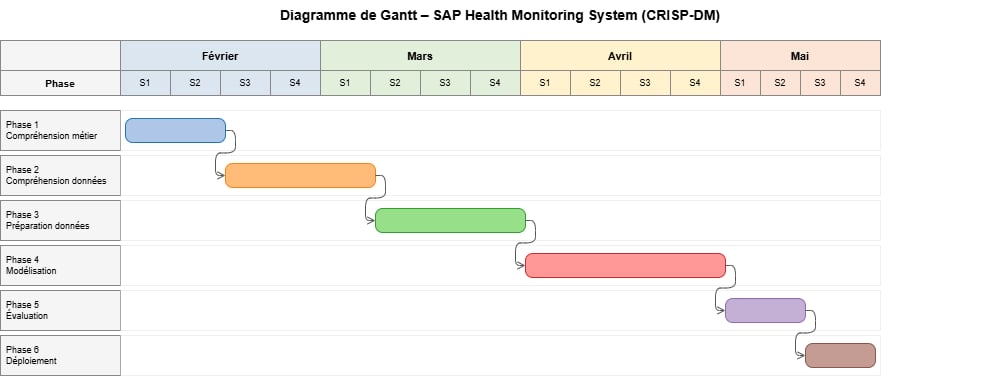
\includegraphics[width=\textwidth]{images/diagramme-de-gant.jpeg}
    \caption{Diagramme de Gantt }
    \label{fig:gantt}
\end{figure}

\section*{Conclusion}
\addcontentsline{toc}{section}{Conclusion}

Ce chapitre a posé l'ensemble des fondements du projet selon la phase Business Understanding de CRISP-DM~: contexte métier SAP et rôle du consultant BASIS, vision et objectifs de la solution, acteurs et besoins fonctionnels et non fonctionnels chiffrés, état de l'art des architectures d'IA générative (Fine-Tuning, RAG, CAG), choix d'une approche RAG hybride enrichie par cache, et planification temporelle du projet selon les six phases CRISP-DM. Le chapitre suivant aborde la phase Data Understanding en présentant les sources documentaires SAP et leur qualité.
